\chapter{Fejlesztői dokumentáció} % Developer guide
\label{ch:impl}

\section{Webalkalmazás specifikáció}
Az alkalmazás fő célja egy olyan működő webáruház bemutatása, ami Angular keretrendszer segítségével készült. A webalkalmazás két főrészre osztható kliensoldali és szerveroldali (szakmai nyelven kifejezve: front-end és back-end) részre. A kliensoldal leglényegesebb feladata, hogy a felhasználó által is látott weboldalt megjelenítse grafikai UI/UX(rövidítés feloldása: User interface/User experience)dizájn implementálásával. Nevezetesen egy olyan rendszer, ami képes a felhasználó számára felületet és élményt biztosítani. Miközben a szerveroldal elsődleges feladata az alkalmazás úgynevezett business logikájának a megvalósítása. Ezen felül képes az adatok feldolgozására és hitelesítésére is. A következő ábrán szeretném reprezentálni milyen módon épül fel a webalkalmazás, továbbá megismertetni a két oldal kommunikációs kapcsolatát.

\begin{figure}[H]
	\centering
	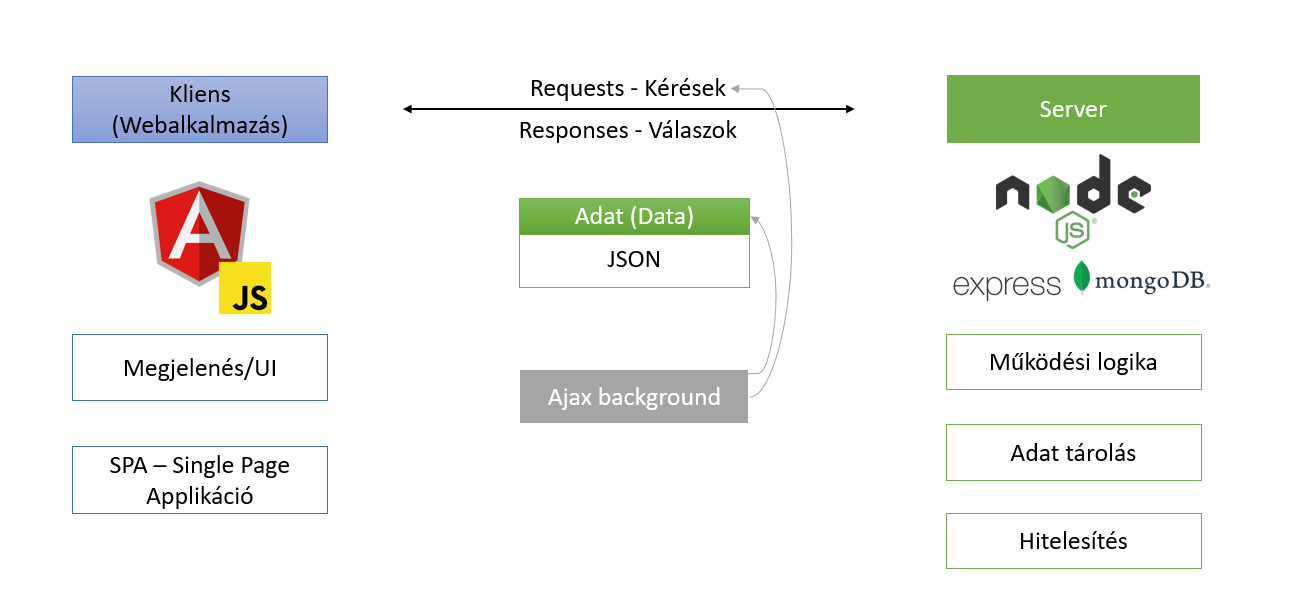
\includegraphics[width=1.0\textwidth,height=250px]{images/alkalmazas_bemutatasa.png}
	\caption{Az alkalmazás bemutatása}
	\label{fig.picture-1}
\end{figure}

A 3.1-es ábrán látható a két oldal miképpen osztja meg az információkat egymás között. A front-end pontosabban mondva a kliensoldal Angular keretrendszerben TypeScript segítségével íródott. A front-end kommunikációja úgynevezett requestekkel más néven kérésekkel (json típusú adattovábbítással) a háttérben aszinkron módon történik amire a szerveroldal responsokkal egyszóval válaszokkal felel. A back-end Node.js szoftverrendszer alapú, ami Express segítségével íródott. Az adatok tárolásáért a MongoDB nevezetű adatbázis felel.

\bigskip
A következő blokkokban szeretném tételesen demonstrálni a fentebb említett front-end és back-end oldalakon használt módszerek alkalmazását és működését. Ezen felül szándékomban áll ismertetni az általam alkalmazott szoftverek technikai tulajdonságaikat.

\section{Kliensoldalon használt technológiák bemutatása}
A dokumentáció és az egész program fő eleme az Angular keretrendszer, aminek a segítségével dinamikus webalkalmazások hozhatóak létre. Az Angular egy nyílt forráskódú a Google által fejlesztett JavaScript nyelven írt front-end keretrendszer. Ebben a fejezetben szeretném kellőképpen kifejteni miért ezt a rendszert választottam az alkalmazás megírásához ezen felül alaposabban bemutatni a működését és főbb tulajdonságait. 

\begin{figure}[H]
	\centering
	
\includegraphics[width=1.0\textwidth,height=250px]{images/angular_bemutatas.png}
	\caption{Az Angular keretrendszer bemutatása}
	\label{fig.picture-2}
\end{figure}

 egy kliensoldali keretrendszerről beszélhetünk
 képes megjeleníteni a back-end felől érkező adatokat
 a felhasználó által beérkezett adatokat képes feldolgozni, kezelni
 képes a szerveroldallal kapcsolatot létesíteni
 biztosítja a ui/ux feluletet a felhasználó számára
A program megírása során a 13.0.4 legújabb verziójú Angular CLI került telepítésre.

\section{Kliensoldal működése}

\section{Szerveroldalon használt technológiák bemutatása}
A szerveroldalon használt (3.1-es blokkban már említésre kerülő) módszerek kiválasztásuk előtt kulcsfontosságú szempontjuknak tartottam, hogy az Angular keretrendszerhez megfelelő kompatibilitással rendelkezzenek és alkalmazni tudjam őket a szakdolgozat elkészítése során. A következő technológiák mind olyan szoftverek, frameworkök vagy szerverek amikhez számtalan monográfia elérhető az interneten, ezzel támogatva a későbbiekben létrehozott projekteket. A következő felsorolásban összefoglalásképpen összegyűjtöttem az alkalmazásban fellelhető általam használt szoftvereket és verziószámukat:

\begin{itemize}
	\item Node.js: 14.15.4
	\item Express.js: 4.17.1
	\item Mongoose: 6.0.12
	\item MongoDB Atlas
\end{itemize}

\bigskip
A fejezet további részében szeretném ismertetni a fentebb felsorolt technológiák jellegzetes tulajdonságaikat, főbb jellemzőiket további ábrák segítségével.

\subsection{Node.js szoftverrendszer}

\begin{figure}[H]
	\centering
	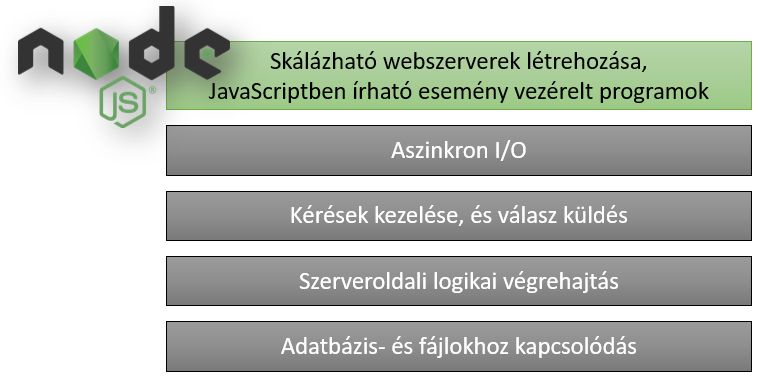
\includegraphics[width=1.0\textwidth,height=220px]{images/nodejs_bemutatasa.png}
	\caption{NodeJS bemutatása}
	\label{fig.picture-3}
\end{figure}

A webáruház back-end megírásánál 14.15.4-es verziójú Node.js szoftverrendszert használtam. A 3.2-es ábrán látható a Node.js bemutatása, ami összefoglalja a szoftverrendszer fontosabb jellemzőit. Az illusztráció első dobozában olvasható miszerint a Node.js skálázható webszerverek létrehozására alkalmas más szóval egy olyan rendszert tudunk létrehozni a támogatásával, ami több felhasználót képes egyidejűleg kiszolgálni. Ezenfelül JavaScript nyelv segítségével olyan programok írhatóak, amely a komponensek közötti esemény interakciókat tekinti alapul, mászóval eseményvezérelt programok megírására alkalmas (ilyen például egy egérkattintás vagy billentyű leütés). Folytatólag a Node.js aszinkron tulajdonságával lehetővé teszi, hogy a kliensoldalról érkező kérések várakozási sorrendbe kerüljenek, ennek következtében a kliensoldal tovább folytathatja a feladatát. 

\subsection{Express.js framework és Mongoose programozási könyvtár}

\begin{figure}[H]
	\centering
	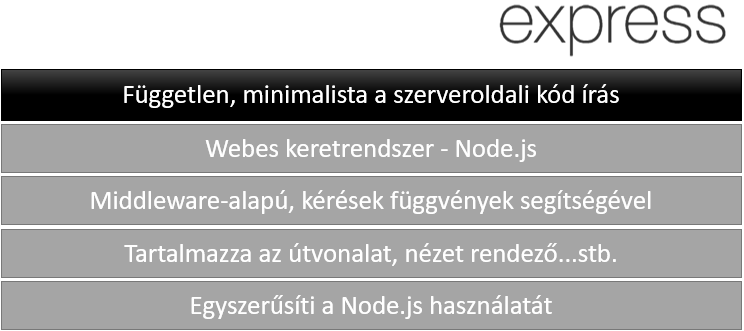
\includegraphics[width=0.8\textwidth,height=220px]{images/express_bemutatasa.png}
	\caption{Express bemutatása}
	\label{fig.picture-4}
\end{figure}

A szerveroldal áttekinthetőbb és olvashatóbb kódírása érdekében a webáruház fejlesztése során az Express.js 4.17.1-es verzióját használtam. Az Express egy webes keretrendszer a Node.js nehézség nélküli használatára lett fejlesztve. A 3.3-as ábrán látható az Express attribútumainak ismertetése. Az illusztráción felvetettem, hogy az Express egy Middleware-típusú rendszer következésképpen lehetővé teszi a MongoDB adatbázis szoftverhez való zavartalan kapcsolódást a Mongoose 6.0.12 verziójával kiegészítve, ami egy JavaScript-ben írt objektum-orientált programozási könyvtár.

\subsection{MongoDB adatbázisszerver}

\begin{figure}[H]
	\centering
	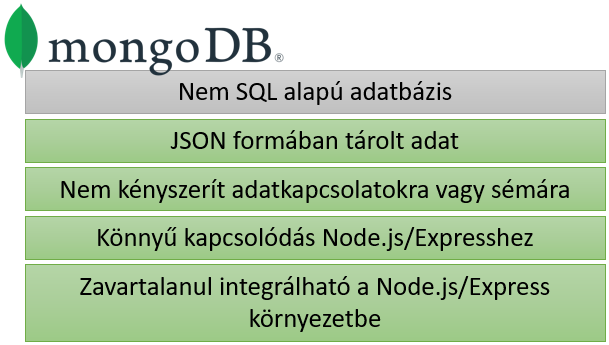
\includegraphics[width=0.8\textwidth,height=220px]{images/mongodb_bemutatasa.png}
	\caption{MongoDB bemutatása}
	\label{fig.picture-5}
\end{figure}

A MongoDB egy nyílt forráskódú, NoSQL adatbázisszerverek közé sorolt szoftver. A NoSQL magyarán Nem SQL típusú adatbázisrendszert jelent. Jellemzően nem rekordokat és táblázatokat tárolnak mint az SQL típusú szerverek, hanem független dokumentumokat és gyűjteményeket archiválnak. Személyes véleményem szerint a 3.4-es illusztrációval alátámasztva egyik legfőbb pozitív tulajdonságának éreztem a alkalmazás írása során, hogy az adatok JSON formátumban képes tárolni. Következésképpen a request és response folyamatok egyszerűsített és gyors működését képes biztosítani, mindeközben lehetővé teszi a kliensoldalon megjelenítendő információk könnyebb feldolgozását. 
\bigskip

\subsection{NoSQL vs SQL adatbázisok összehasonlítása}

A következő grafikai ábrán szándékozom röviden bemutatni és összehasonlítani a Nem SQL és az SQL alapú adatbázisokat jellegzetes tulajdonságaik szerint.

\begin{figure}[H]
	\centering
	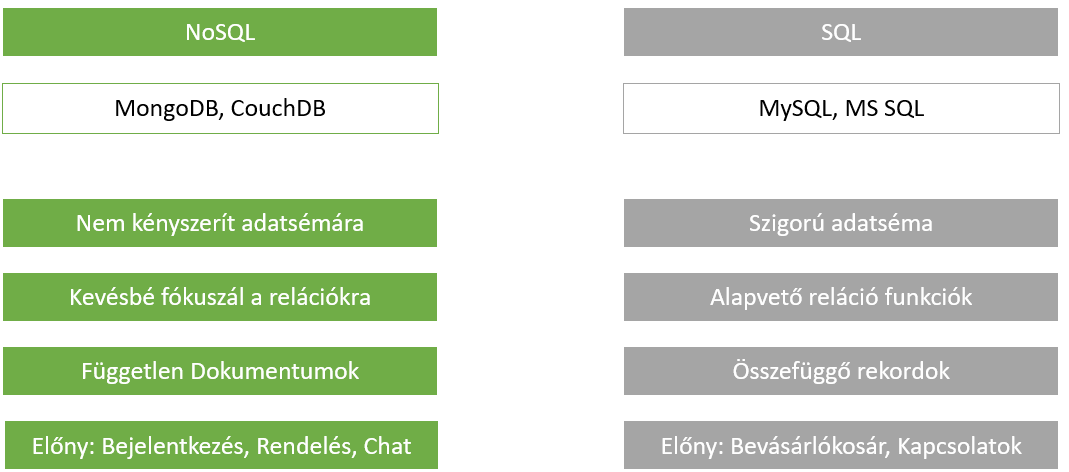
\includegraphics[width=1.0\textwidth,height=220px]{images/nosql_bemutatasa.png}
	\caption{NoSQL vs SQL adatbázisok összehasonlítása}
	\label{fig.picture-6}
\end{figure}

Mint a 3.5-ös ábrán megfigyelhető szempontok szerint egy webáruházban kezelt adatok tárolására a No SQL adatbázisok is kifejezetten alkalmasok. A NoSQL adatbázisszerverek jellemző tulajdonságai kulcsfontosságú szempontokkal szolgált a webáruház adatbázisának kiválasztásánál.

\section{Szerveroldal működése}

Ebben a fejezetben részletesen prezentálom az alkalmazás szerveroldali működését példának okáért milyen request és response hívások találhatóak a kódban, hogyan létesít kapcsolatot a webalkalmazás az adatbázissal...stb., valamint külön kitérek az admin oldalon található hitelesítésre alkalmazott technikára is.

\subsection{RESTful API - Végpont tervek bemutatása}

A webáruház megírása során RESTful API-t (feloldva: Representational State Transfer Application programming interface) magyarán reprezentáción alapuló állapotátvitel nevezetű architekturális módszert használtam. Az API-k segítségével a felhasználó számára elérhető a weboldalon számos interakció. Ilyen interakciónak számít például a bejelentkező felület.

\bigskip
Az alábbi illusztráción szeretném bemutatni az alkalmazásban használt REST API hívásokat, ennek okán a 3.6-os ábrán láthatók a programban megírt végpontok.


\begin{figure}[H]
	\centering
	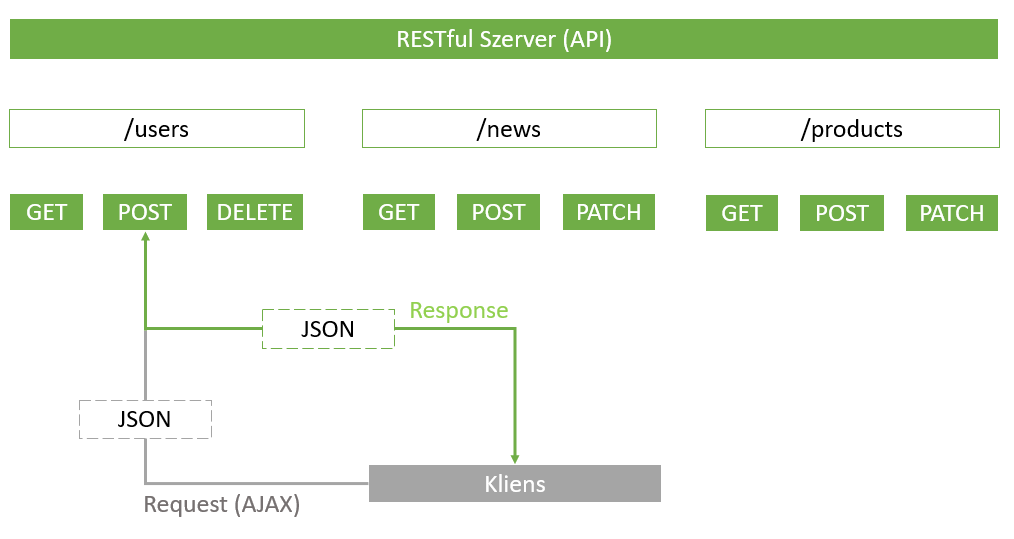
\includegraphics[width=1.0\textwidth,height=220px]{images/restapi_bemutatasa.png}
	\caption{Adatkezelés}
	\label{fig.picture-8}
\end{figure}

 A grafikán megfigyelhető hét különböző végpont ami az auth, hírek, termékek, termékcsoportok, üzenetek, chatek és rendeléseket fejezi ki. Az illusztrációt figyelemmel kísérve identifikálható, hogy nem minden végpont rendelkezik ugyan azokkal a kérésekkel. Szemléltetésképp vegyük figyelembe a hírekhez vonatkozó responsokat amik a GET, POST, PATCH és DELETE függvények, ezzel szemben a auth-hoz kizárólag POST függvény tartozik. Ennek kifejezetten egy oka van, mégpedig az, hogy a webáruház egyes adatait nem szükséges módosítani tudni kliens oldalról.

\bigskip
A REST API-t megismerve és ezt az információt felhasználva szemléltethető és az alább ábrán látható miképpen éri el a felhasználó által kezdeményezett kérés az adatbázist és hogyan kerül válaszra.

\begin{figure}[H]
	\centering
	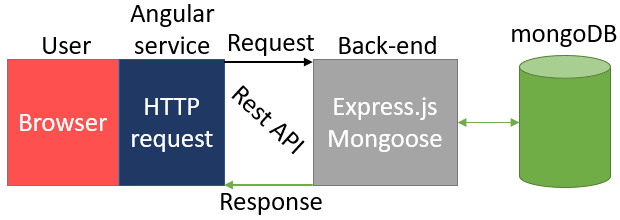
\includegraphics[width=1.0\textwidth,height=220px]{images/kapcsolat_szerver_bemutatas.png}
	\caption{Kapcsolat a szerverrel}
	\label{fig.picture-7}
\end{figure}

A fenti 3.7-es ábrával és az alább található alkalmazásban szereplő kódsorok segítségével szeretném bemutatni, hogy a felhasználó által indított kérés milyen sorrendben jut el az adatbázishoz és miképpen tér vissza hozzá.

\bigskip
Felhasználó interakcióba lép a felülettel (például: egy gombra kattintva~\ref{src:html}-es forráskód), ennek következményeként meghívódik egy a gombhoz tartozó TypeScript nyelven írt függvény \ref{src:ts}-es forráskód.

\lstset{caption={Felhasználói interakció - HTML fájl}, label=src:html}
\begin{lstlisting}[language=html]
	<form style="margin-top: 2rem;" [formGroup]="form" (submit)="onAddMessage()" *ngIf="!isLoading">
	....
	<button class="btn-secondary" type="submit" [disabled]="!confirmed.checked">
		{{'GENERIC.ACTION.SEND' | translate}}
	</button>
\end{lstlisting}

\lstset{caption={Interakció függvényhívás - TypeScript fájl}, label=src:ts}
\begin{lstlisting}[language=JavaScript]
	onAddMessage(): void {
		if(this.form.invalid) {
			this.alertService.warn('ALERT.WARN.INVALID_FORM');
			this.form.markAllAsTouched();
			this.isLoading = false;
			return;
		}
		this.isLoading = true;
		this.contactService.sendMessage(
			this.form.value.firstName,
			this.form.value.lastName,
			this.form.value.email,
			this.form.value.description,
			this.form.value.image,
		)
		this.isLoading = false
		this.form.reset();
	}
\end{lstlisting}

Az előbb említett \ref{src:ts}-es forráskódban szereplő függvény átadja az adatokat a kliensoldalon található Service fájl sendMessage() nevezetű függvényének. Ez a fájl tartalmazza a következő \ref{src:service}-as forráskódban szereplő kódsort.

\lstset{caption={HttpClient POST request - Service TypeScript fájl}, label=src:service}
\begin{lstlisting}[language=JavaScript]
	sendMessage(
		firstName: string, 
		lastName: string, 
		email: string, 
		description: string, 
		image: File | string
	){
		const messagesData = new FormData();
		messagesData.append("firstName", firstName);
		messagesData.append("lastName", lastName);
		messagesData.append("email", email);
		messagesData.append("description", description);
		messagesData.append("image", image, firstName);
		this.http.post<{message: string, messages: Messages}>
		(environment.apiUrl + "messages", messagesData)
			.subscribe(responseData => {
				const messages: Messages = {
					id: responseData.messages.id,
					firstName: firstName,
					lastName: lastName,
					email: email,
					description: description,
					imagePath: responseData.messages.imagePath,
				};
				this.messages.push(messages);
				this.msgUpdate.next([...this.messages]);
				this.alert.success('ALERT.SUCCESS.ADD');
				this.router.navigate(["/contact"]);
			}, error => {
				this.alert.error(error.error.message);
			});
	}
\end{lstlisting}

Ebben a kódrészletben látható, ahogyan a kliens oldal HttpClient Angular package POST request segítségével a megadott útvonalon küld egy REST API kérést a szerveroldal felé.

\bigskip
A szerveroldal fogadja ezt a kérést és továbbítja a MongoDB felé. Az alábbi \ref{src:express}-es forráskódban Express - JavaScript nyelv segítségével megírt kódrészletben ez szerepel.

\lstset{caption={Express POST végpont - JavaScript}, label=src:express}
\begin{lstlisting}[language=JavaScript]
	exports.postMessages = (req, res, next) => {
		const url = req.protocol + "://" + req.get("host");
		const msg = new Messages({
			firstName: req.body.firstName,
			lastName: req.body.lastName,
			email: req.body.email,
			description: req.body.description,
			imagePath: url + "/images/messages/" + req.file.filename,
		});
		msg.save().then(result => {
			res.status(201).json({
				message: "Message added successfully",
				messages: {
					...result,
					id: result._id
				}
			});
		});
	}
\end{lstlisting}

Kliensoldalon és Szerveroldalon egyaránt látható a felhasználó által elindított kérés státuszát tartalmazó információ. A front-end-en egy úgynevezett AlertService componens segítségével kap visszaigazolást az elindított kérés befejezéséről, míg a back-end-en az adatbázis felé elküldött kérés kódrészletében található ez az információ.

\bigskip
A webalkalmazásban szereplő további REST API hívásokat tartalmazó példakódsorokat a 3.7-es Forráskódok 3.7.2-es Szerveroldali forráskódok nevezetű alfejezetben találhatóak.

\subsection{Hitelesítés - Admin felület védelme}
Az alkalmazás megírása során akaratlagosan egy olyan webáruház létrehozása volt a végcélom, ami időszerű adatok kezelését tudja biztosítani. Következésképpen egy olyan felület megvalósítása gyakorlatban is, amely nem igényel programozón keresztüli beavatkozást. Ennek okán a szakdolgozat tartalmaz egy adminisztrációs oldalt, amely biztosítja a webalkalmazásban dinamikusan megjelenő adatok aktualitását, továbbá a leadott rendelések vásárlók által elküldött üzenetek megjelenítésére is szolgál. Kifejezetten ennek a blokk védelmében került bele külön hitelesítési felület.

\bigskip
Az alább található 3.8-as grafikán ez az engedélyezési folyamat elméleti működése látható.
 
\begin{figure}[H]
	\centering
	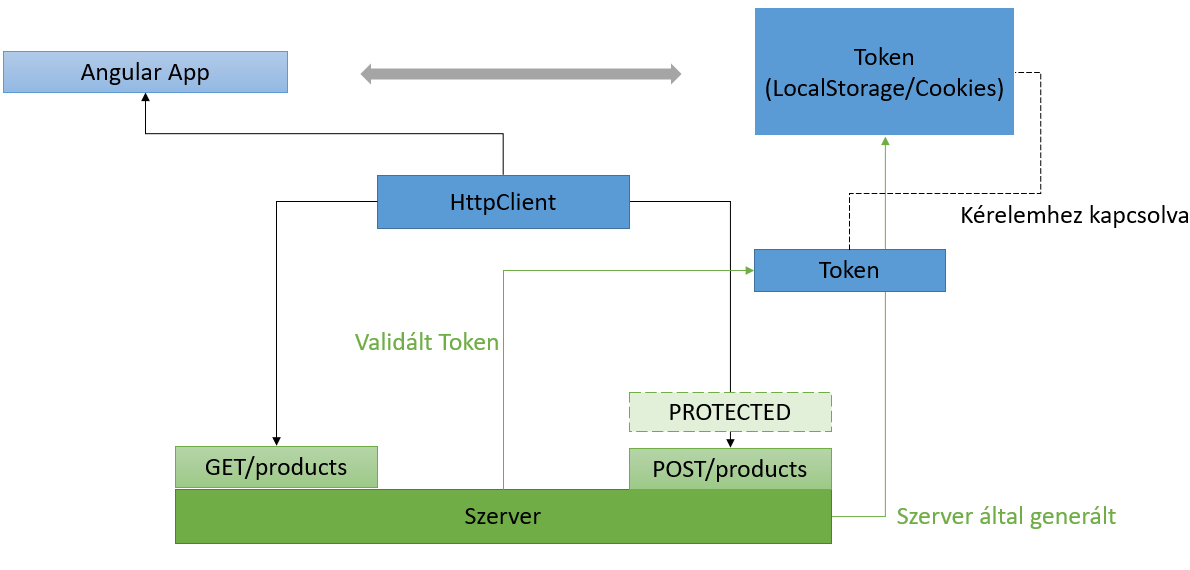
\includegraphics[width=1.0\textwidth,height=220px]{images/hitelesites_bemutatasa.png}
	\caption{Hitelesítés}
	\label{fig.picture-9}
\end{figure}

Az illusztráción ábrázolt hitelesítési folyamat a következőképpen történik. Az alkalmazás front-end-ről érkező GET/products kérésre engedélyezés nélkül kap választ a szervertől, mivel a webáruházban bejelentkezés hiányában is hozzáférhetővé kell tenni ezt az információt. Ezzel szemben a POST/products kérés nem következhet be hitelesítés nélkül. Tehát bejelentkezés során a szerver generál egy úgynevezett tokent és LocalStorage-ba elmenti, amit az új termék hozzáadás kérésnél ellenőriz. Az alkalmazásban ez a hitelesítési funkciót következőképpen valósul meg:

Ennek a funkciónak létrehozásánál két kiegészítő package-et úgynevezett bcryptjs-t és jsonwebtoken-t használja a programkód. Az előbbi lehetőséget nyújt bizonyos adatok titkosítására (ilyen adat például a belépési jelszó), az utóbbi pedig bizonyos REST API kérések érvényesítésére alkalmas. Mikor létrehozásra kerül egy új felhasználó a bcrypt package egy úgynevezett hash metódusát hívja meg a program, aminek segítéségével az új felhasználó jelszava titkosítva kerül be az adatbázisba. Ennek oka az, hogy ha véletlenül sikerül egy idegennek belépnie az adatbázisba, akkor ne tudja megszerezni az adott felhasználók jelszavát. Viszont, ha titkosítva kerül be az adat, a későbbiekben belépésnél nem lehet ellenőrizni, hogy a megfelelő jelszó került-e beírásra. Erre a problémára szolgál megoldásképp a bcryptjs compare metódusának használata, aminek segítségével összehasonlításra kerül az adott felhasználó adatbázisban szereplő jelszava és a begépelt jelszó hashelt változata, mivel ha pont a megfelelő adat kerül beírásra akkor a titkosított információnak megegyezőnek kell lennie az adatbázisban található jelszóval. Sikeres bejelentkezésnél a szerveroldal generál egy tokent a jsonwebtoken package segítségével és minden olyan kérésnél amihez szükséges autentikáció, ellenőrzésre kerül ennek az érvényes tokennek a létezése. A programkódban generált tokenek hitelessége egy óráig él.

\bigskip
Mindent összevetve az adminisztrációs felület védve van az illetéktelen felhasználók belépésétől és bizonyos funkciók végrehajtásától. A hitelesítési folyamatot leíró példakódok a 3.7-es Forráskódok, 3.7.2-es Szerveroldali forráskódok nevezetű alfejezetben találhatóak.

\section{Fogalomtár, megjegyzések} % Theorem-like items

\begin{definition}
Mauris tristique sollicitudin ultrices. Etiam tristique quam sit amet metus dictum imperdiet. Nunc id lorem sed nisl pulvinar aliquet vitae quis arcu. Morbi iaculis eleifend porttitor.
\end{definition}

Maecenas rutrum eros sem, pharetra interdum nulla porttitor sit amet. In vitae viverra ante. Maecenas sit amet placerat orci, sed tincidunt velit. Vivamus mattis, enim vel suscipit elementum, quam odio venenatis elit, et mollis nulla nunc a risus. Praesent purus magna, tristique sed lacus sit amet, convallis malesuada magna. Phasellus faucibus varius purus, nec tristique enim porta vitae.

\begin{theorem}
Nulla finibus ante vel arcu tincidunt, ut consectetur ligula finibus. Mauris mollis lectus sed ipsum bibendum, ac ultrices erat dictum. Suspendisse faucibus euismod lacinia. Etiam vel odio ante.
\end{theorem}
\begin{proof}
Etiam pulvinar nibh quis massa auctor congue. Pellentesque quis odio vitae sapien molestie vestibulum sit amet et quam. Pellentesque vel dui eget enim hendrerit finibus at sit amet libero. Quisque sollicitudin ultrices enim, nec porta magna imperdiet vitae. Cras condimentum nunc dui.
\end{proof}

Donec dapibus sodales ante, at scelerisque nunc laoreet sit amet. Mauris porttitor tincidunt neque, vel ullamcorper neque pulvinar et. Integer eu lorem euismod, faucibus lectus sed, accumsan felis. 

\begin{remark}
Nunc ornare mi at augue vulputate, eu venenatis magna mollis. Nunc sed posuere dui, et varius nulla. Sed mollis nibh augue, eget scelerisque eros ornare nec. Praesent porta, metus eget eleifend consequat, eros ligula eleifend ex, a pellentesque mi est vitae urna. Vivamus turpis nunc, iaculis non leo eget, mattis vulputate tellus.
\end{remark}

Fusce in aliquet neque, in pretium sem. Donec tincidunt tellus id lectus pretium fringilla. Nunc faucibus, erat pretium tempus tempor, tortor mi fringilla neque, ac congue ex dui vitae mauris. Donec pretium et quam a cursus.

\begin{note}
Aliquam vehicula luctus mi a pretium. Nulla quam neque, maximus nec velit in, aliquam mollis tortor. Aliquam erat volutpat. Curabitur vitae laoreet turpis. Integer id diam ligula.
\end{note}

Ut sollicitudin tempus urna et mollis. Aliquam et aliquam turpis, sed fermentum mauris. Nulla eget ex diam. Donec eget tellus pharetra, semper neque eget, rutrum diam.


\section{Forráskódok} % Source code samples

\subsection{Kliensoldali forráskódok}
Nulla sodales purus id mi consequat, eu venenatis odio pharetra. Cras a arcu quam. Suspendisse augue risus, pulvinar a turpis et, commodo aliquet turpis. Nulla aliquam scelerisque mi eget pharetra. Mauris sed posuere elit, ac lobortis metus. Proin lacinia sit amet diam sed auctor.

\subsection{Szerveroldali forráskódok}
Alább található forráskódok a 3.5.1-es fejezetben megemlített JavaScriptben írt egy-egy példa request végpontokat tartalmaz.

POST/news~\ref{src:post} és a visszaérkező json fájl \ref{src:postJson}:

\lstset{caption={POST/news végpont}, label=src:post}
\begin{lstlisting}[language=JavaScript]
exports.postNews = (req, res, next) => {
	const url = req.protocol + "://" + req.get("host");
	const news = new News({
		title: req.body.title,
		description: req.body.description,
		imagePath: url + "/images/news/" + req.file.filename,
		startDate: req.body.startDate,
		endDate: req.body.endDate,
	});
	news.save().then(result => {
		res.status(201).json({
			message: "News added successfully",
			news: {
				...result,
				id: result._id
			}
		});
	});
}
\end{lstlisting}

\lstset{caption={POST/news JSON}, label=src:postJson}
\begin{lstlisting}[language={JSON}]
{
	"_id":
	{
		"$oid":"618e7a2edd33576f6e96b11c"
	},
	"title":"Teszt",
	"description":"Teszt szoveg",
	"imagePath":"http://localhost:3000/images/news/teszt-1636727342360.jpg",
	"startDate":
	{
		"$date":
		{
			"$numberLong":"1637276400000"
		}
	},
	"endDate":
	{
		"$date":
		{
			"$numberLong":"1637881200000"
		}
	}
\end{lstlisting}

Az alábbi forráskódok a 3.5.2-es alfejezetben kifejtett hitelesítési funkció kódbeli megvalósítása olvasható. Ezen programkódok részben Maximilian Schwarzmüller által írt kód felhasználásával történt.




\subsection{Algoritmusok} % Algorithms

A general Interval Branch and Bound algorithm is shown in Algorithm~\ref{alg:ibb}. One of the following selection rules is applied in Step \ref{step:selrule}.\\
Példa forrása: \href{https://www.inf.u-szeged.hu/actacybernetica/}{Acta Cybernetica (ez egy link)}.

\begin{algorithm}[H]
\caption{A general interval B\&B algorithm} 
\label{alg:ibb} 
\textbf{\underline{Funct}} IBB($S,f$)
\begin{algorithmic}[1] % sorszámok megjelenítése minden n. sor előtt, most n = 1
\State Set the working list ${\cal L}_W$ := $\{S\}$ and the final list ${\cal L}_Q$ := $\{\}$     
\While{( ${\cal L}_W \neq \emptyset$ )} \label{alg:igoend}
	\State  Select an interval $X$ from ${\cal L}_W$ \label{step:selrule}\Comment{Selection rule}  
	\State Compute $lbf(X)$ \Comment{Bounding rule}		  
	\If{$X$ cannot be eliminated} \Comment{Elimination rule}
		\State Divide $X$ into $X^j,\ j=1,\dots, p$, subintervals   \Comment{Division rule}
		\For{$j=1,\ldots,p$}
			\If{$X^j$ satisfies the termination criterion} \Comment{Termination rule}
				\State Store $X^j$ in ${\cal L}_W$ 
			\Else
				\State Store $X^j$ in ${\cal L}_W$ 
			\EndIf
		\EndFor  
	\EndIf
\EndWhile
\State \textbf{return} ${\cal L}_Q$
\end{algorithmic}
\end{algorithm}

\section{Tesztesetek}

\section{Továbbfejlesztési lehetőségek}